\documentclass[t]{beamer}
\usefonttheme{serif}

\usepackage{amsmath,amsthm,amssymb,amsfonts,amscd,mathrsfs,amsxtra,multirow,kotex,mathtools,gensymb,textcomp,lipsum,tikz,verbatim,color,soul,courier,mdframed,xcolor}
\usepackage[normalem]{ulem}
\usetikzlibrary{calc,matrix,arrows,chains,positioning,scopes}
\usepackage{pdfpages,cancel}

\theoremstyle{plain}
\newtheorem{thm}{Theorem}[section]
\newtheorem{prop}[thm]{Proposition}

\theoremstyle{definition}
\newtheorem{defn}[thm]{Definition}
\newtheorem{exmp}[thm]{Example}
\newtheorem{excs}[thm]{Exercise}
\newtheorem{rem}[thm]{Remark}
\newtheorem{prob}[thm]{Problem}
\newtheorem{cor}[thm]{Corollary}

\newcommand \tr[1]{\textcolor{red}{#1}}
\newcommand{\tikzmark}[1]{\tikz[overlay,remember picture] \node (#1) {};}
\newcommand{\varep}{\varepsilon}
\newcommand{\DrawBox}[1][]{%
    \tikz[overlay,remember picture]{
    \draw[red,#1]
      ($(left)+(-0.2em,0.9em)$) rectangle
      ($(right)+(0.2em,-0.3em)$);}
}

\newcommand{\tikzmarkk}[2]{
    \tikz[overlay,remember picture,baseline] 
    \node[anchor=base] (#1) {$#2$};
}
\newcommand*\circled[1]{\tikz[baseline=(char.base)]{
            \node[shape=circle,draw,inner sep=2pt] (char) {#1};}}

\tikzset{join/.code=\tikzset{after node path={%
\ifx\tikzchainprevious\pgfutil@empty\else(\tikzchainprevious)%
edge[every join]#1(\tikzchaincurrent)\fi}}}

\tikzset{>=stealth',every on chain/.append style={join},
         every join/.style={->}}
\tikzstyle{labeled}=[execute at begin node=$\scriptstyle,
   execute at end node=$]

\newenvironment<>{proofs}[1][\proofname]{%
   \par
   \def\insertproofname{#1\@{.}}%
   \usebeamertemplate{proof begin}#2}
 {\usebeamertemplate{proof end}}
 

\addtobeamertemplate{navigation symbols}{}{%
    \usebeamerfont{footline}%
    \usebeamercolor[fg]{footline}%
    \hspace{1em}%
    \raisebox{2pt}[0pt][0pt]{\insertframenumber/\inserttotalframenumber}
}
\setbeamercolor{footline}{fg=blue}
\setbeamerfont{footline}{series=\bfseries}
\title[]{SE102:Multivariable Calculus}

\author[]{Hyosang Kang\inst{1}}

\institute[]{\inst{1}Division of Mathematics\\ School of Interdisciplinary Studies\\ DGIST}

\date[]{Lecture 06\\
Line and Surface Integrals}

\begin{document}

\begin{frame}
\titlepage
\end{frame}

\begin{frame}
\begin{defn}\label{defn-Jacobian}
Let $D,R$ be regions in $\mathbf R^n$.
A differentiable one-to-one function $T:R\to D$ 
is called a \textbf{transformation}.
For $T(u_1,\cdots,u_n) = (x_1,\cdots,x_n)$, 
the \textbf{Jacobian} of $T$ is defined as the determinant of the differential of $T$:
	$$J_T = \det \mathbf dT.$$
We also denoted $J_T$ as
	$$J_T = \frac{\partial(x_1,\cdots,x_n)}{\partial(u_1,\cdots,u_n)}$$
\end{defn}
\end{frame}

\begin{frame}
\begin{thm}[Integration by substitution]
Let $T:R\to D$ be a transformation, 
and $f(x,y)$ be a continuous function defined on $D$.
Then
	$$\iint_Df(x,y)dxdy=\iint_R(f\circ T)(u,v)|J_T|dudv.$$
\end{thm}
\begin{rem}
It is useful to remember the subsitution rule as:
	$$\iint_Df(x,y)dxdy
	= \iint_R(f\circ T)(u,v)\left|\frac{\partial(x,y)}{\cancel{\partial(u,v)}}\right|\cancel{dudv}$$
Also, the Jacobian of the inverse $T^{-1}(x,y)=(u(x,y),v(x,y))$ is
	$$J_{T^{-1}}=\left|\frac{\partial(u,v)}{\partial(x,y)}\right|
	=\frac{1}{J_T}=\frac{1}{\left|\frac{\partial(x,y)}{\partial(u,v)}\right|}$$
\end{rem}
\end{frame}

\begin{frame}
\begin{exmp}
Compute
	$$\iint_D |x|e^{-x^2-y^2}dxdy$$
where $D=\{(x,y)\,|\,x^2+y^2\le1\}$.
\end{exmp}
\end{frame}

\begin{frame}
\begin{thm}[Integration by substitution]
Let $V,W$ be regions in $\mathbf R^3$.
A differentiable one-to-one function $T:W\to V$ 
	$$T(u,v,w) = (x(u,v,w),y(u,v,w),z(u,v,w))$$
is called a \textbf{transformation}.
Let $f(x,y,z)$ be a continuous function on $V$.
Then
	$$\iiint_Vf(x,y,z)dxdydz=\iiint_W(f\circ T)(u,v,w)|J_T|dudvdw.$$
\end{thm}
\end{frame}

\begin{frame}
\begin{exmp}
Compute the volume between two cylinders $x^2+y^2\le 1$, $y^2+z^2\le 1$.
	\begin{figure}
	\begin{center}
	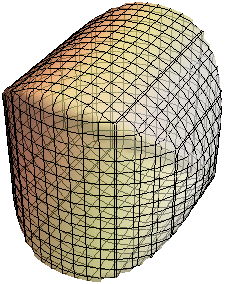
\includegraphics[scale=.25]{image/lnsec10-1}
	\end{center}
    \end{figure}
\end{exmp}
\begin{exmp}
Compute
	$$\iiint_V\sqrt{x^2+y^2+z^2}e^{x^2+y^2+z^2}dxdydz$$
where $V$ is the region between the spheres $x^2+y^2+z^2=a^2$ and $x^2+y^2+z^2=b^2$ ($0<a<b$).
\end{exmp}
\end{frame}

\begin{frame}
\begin{defn}
	A \textbf{vector field} $\mathbf F:\mathbf R^n\to V$
	is a map  which assign a vector in a vector space $V$
	to each point in the space $\mathbf R^n$.
	(Usually we take $V$ as $n$-dimensional 
	vector space $\mathbf R^n$.)
\end{defn}

\begin{defn}
	Given a vector field $\mathbf F(x,y,z) = (P(x,y,z), Q(x,y,z), R(x,y,z))$,
	The \textbf{curl} $\nabla\times F$ and \textbf{divergence} $\nabla\cdot\mathbf F$
	is defined by
	\begin{align*}
		\nabla\times\mathbf F &= (R_y-Q_z,P_z-R_x,Qx-P_y) = \left|\begin{matrix} i & j & k \\ \partial/\partial_x & \partial/\partial_y & \partial/\partial_z \\ P & Q & R \end{matrix}\right| \\
		\nabla\cdot\mathbf F &= P_x+Q_y+R_z
	\end{align*}
\end{defn}
\end{frame}

\begin{frame}
\begin{thm}
Let $f,g$ be $3$-dimensional functions
and $\mathbf F$, $\mathbf G$ be $3$-dimensional vector fields. 
The following properties hold.
\begin{enumerate}
\item $\nabla\times(\nabla f)=0$ 
\item $\nabla\cdot(\nabla\times\mathbf F)=0$
\item $\nabla\cdot(\mathbf F+\mathbf G)=\nabla\cdot\mathbf F+\nabla\cdot\mathbf G$
\item $\nabla\times(\mathbf F+\mathbf G)=\nabla\times\mathbf F+\nabla\times\mathbf G$
\item $\nabla\cdot(f\mathbf F)=f\nabla\cdot\mathbf F+\mathbf F\cdot\nabla f$
\item $\nabla\times(f\mathbf F)=f\nabla\times\mathbf F+\nabla f\times\mathbf F$
\item $\nabla\cdot(\mathbf F+\mathbf G)=\mathbf G\cdot(\nabla\times\mathbf F)-\mathbf F\cdot(\nabla\times\mathbf G)$
\item $\nabla\cdot(\nabla f\times\nabla g)=0$
\item Denote $\nabla^2=\nabla\cdot\nabla$. Then
	$$\nabla\times(\nabla\times\mathbf F)=\nabla(\nabla\cdot\mathbf F)-\nabla^2\cdot\mathbf F$$
\end{enumerate}
\end{thm}
\end{frame}

\begin{frame}
\begin{defn}
Let $\mathbf F(x,y)=(P(x,y), Q(x,y))$ be a 
$2$-dimensional vector field.
The \textbf{curl} of $\mathbf F$ is
	$$\textup{curl}\mathbf F = Q_x - P_y.$$
The \textbf{divergence} of $\mathbf F$ is 
	$$\textup{div}\mathbf F = P_x + Q_y.$$
\end{defn}
\end{frame}

\begin{frame}
\begin{defn}
Let $C$ be a curve in $\mathbf R^n$
and $c:[a,b]\to\mathbf R^n$ be a parametrization of $C$.
Given a $n$-dimensional vector field $\mathbf F$ defined on $C$,
the \textbf{line integral} of $\mathbf F$ is defined by
	$$\int_C\mathbf F\cdot d\mathbf s 
	= \int_a^b\mathbf F((c(t)))\cdot c'(t)dt$$	
\end{defn}	
For $2$-dimensional vector field $\mathbf F = (P,Q)$,
the line integral is denoted by
	$$\int_C\mathbf F\cdot d\mathbf s = \int_C Pdx + Qdy.$$
For $3$-dimensional vector field $\mathbf F = (P,Q,R)$,
the line integral is denoted by
	$$\int_C\mathbf F \cdot d\mathbf s = \int_C Pdx + Qdy + Rdz.$$
\end{frame}

\begin{frame}
\begin{defn}
Let $c:[a,b]\to\mathbf R^n$ be a parametrization
of a curve $C$. If $c(a)=c(b)$, the curve is said to be \textbf{closed}.
The line integral over a closed curve is denoted by
$\displaystyle \oint_C$.
\end{defn}
\begin{exmp}
Let $\mathbf A = \displaystyle 
	\left(-\frac{y}{x^2+y^2},\frac{x}{x^2+y^2}\right)$.
Compute the line integral $\displaystyle \oint_C\mathbf A\cdot d\mathbf s$
where $C$ is a unit circle parametrized by counter-clockwise direction.
\end{exmp}
\end{frame}

\begin{frame}
\begin{defn}
Let $X:D\rightarrow S$ be a parametrization of $S$.
If the vector field
	$$\mathbf n
	=\frac{\mathbf X_u\times \mathbf X_v}{\Vert \mathbf X_u\times \mathbf X_v\Vert }$$
is continuous, we say \textbf{$S$ has an orientation}
and $\mathbf n$ is called an \textbf{orientation}.
\end{defn}
\begin{defn}
Let $\mathbf F$ be a $3$-dimensional vector field
defined on a parametrized surface $S$.
The \textbf{surface integral} of $\mathbf F$ over $S$ is defined by
	$$\iint_S\mathbf F\cdot d\mathbf S 
	= \iint_S(\mathbf F\circ X) \cdot\mathbf ndS$$
where $\mathbf n$ is an orientation of $S$.
\end{defn}
\end{frame}

\begin{frame}
\begin{exmp}
Pick an orientation of a unit sphere and 
compute the surface integral of $\mathbf F = \displaystyle
\frac{(x,y,z)}{x^2+y^2+z^2}$.
\end{exmp}	
\end{frame}

\begin{frame}
\begin{prob}
Let $\mathbf F$, $\mathbf G$ be $3$-dimensional vector fields.
Show that the following properties hold. 
\begin{enumerate}
	\item $\nabla\cdot(\mathbf F\times\mathbf G)=\mathbf G\cdot(\nabla\times\mathbf F)-\mathbf F\cdot(\nabla\times\mathbf G)$
	\item $\nabla\times(\nabla\times\mathbf F)=\nabla(\nabla\cdot\mathbf F)-\nabla\cdot \nabla\cdot\mathbf F$
	\item $\nabla\times(\mathbf F\times\mathbf G) = (\nabla\cdot\mathbf G)\mathbf F - (\nabla\cdot \mathbf F)\mathbf G + (\mathbf G\cdot\nabla)\cdot \mathbf F - (\mathbf F\cdot\nabla)\cdot \mathbf G$
\end{enumerate}
\end{prob}
\end{frame}

\begin{frame}
\begin{prob}
Explain geometric meanings of $\nabla\cdot\mathbf F$ and $\nabla\times\mathbf F$.
\end{prob}
\end{frame}

\begin{frame}
\begin{prob}
Find the area of the region bounded by three cylinders
$x^2+y^2\le 1$, $y^2+z^2\le 1$, and $x^2+z^2\le 1$.
\begin{center}
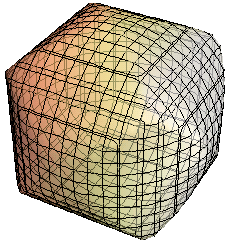
\includegraphics[scale=.25]{image/lnsec10-2}
\end{center}
\end{prob}
\end{frame}

\end{document}